\documentclass[10pt]{jsarticle}

\usepackage[dvipdfmx]{graphicx}
\usepackage{listings}

\setlength{\textwidth}{179mm}
\setlength{\textheight}{251mm}
\setlength{\topmargin}{-2cm}
\setlength{\oddsidemargin}{-1cm}
\setlength{\evensidemargin}{-1cm}

\begin{document}

\begin{titlepage}
\begin{center}\begin{LARGE}
\vspace*{30mm}
\textbf{\Huge REPORT TITLE}\\
\vspace{10mm}
%date 20//()\\
\today\\
\vspace{130mm}
NUMBER NAME\\
\end{LARGE}\end{center}
\end{titlepage}

\section*{section(no number)}
Source code.
\vspace{5mm}
\begin{lstlisting}[basicstyle=\ttfamily\footnotesize, frame=single]
#include <stdio.h>

int main(int argc, char *argv[]) {
    printf("source code here.\n");
    return 0;
}
\end{lstlisting}
\vspace{5mm}
Formula. 
\begin{eqnarray*}
  ax^2 + bx + c &=& 0\\
  x &=& \frac{-b \pm \sqrt{b^2 - 4ac}}{2a}
\end{eqnarray*}

\section{section}
\subsection{subsection}
test figure \ref{fig:1} and \ref{fig:2} with minipage.
\begin{figure}[htbp]
 \begin{minipage}{0.5\hsize}
  \begin{center}
  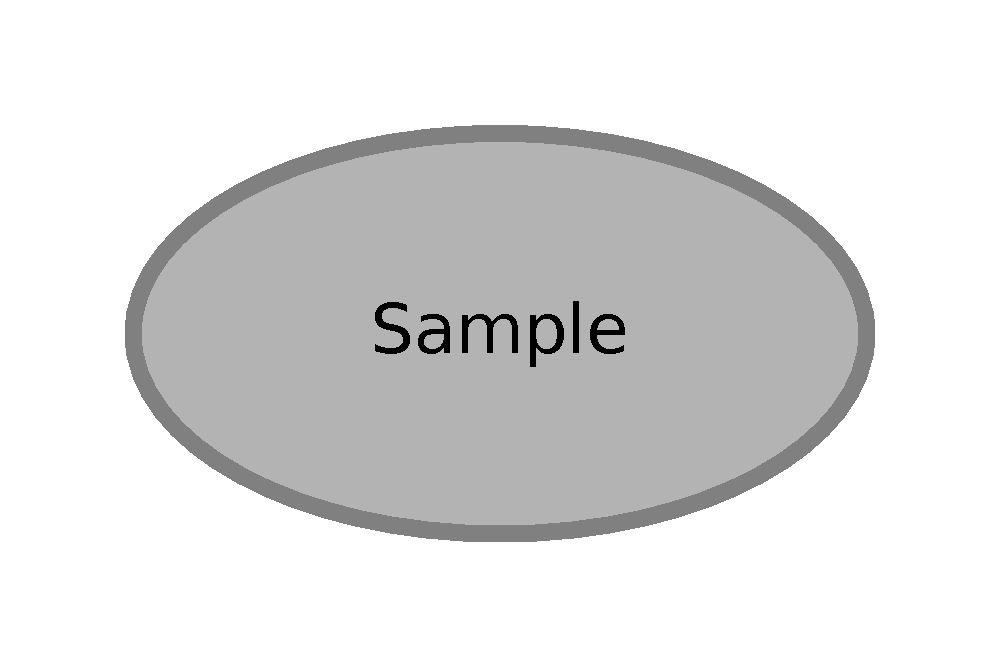
\includegraphics[width=40mm]{sample1.pdf}
  \end{center}
  \caption{sample fig1}
  \label{fig:1}
 \end{minipage}
 \begin{minipage}{0.5\hsize}
  \begin{center}
  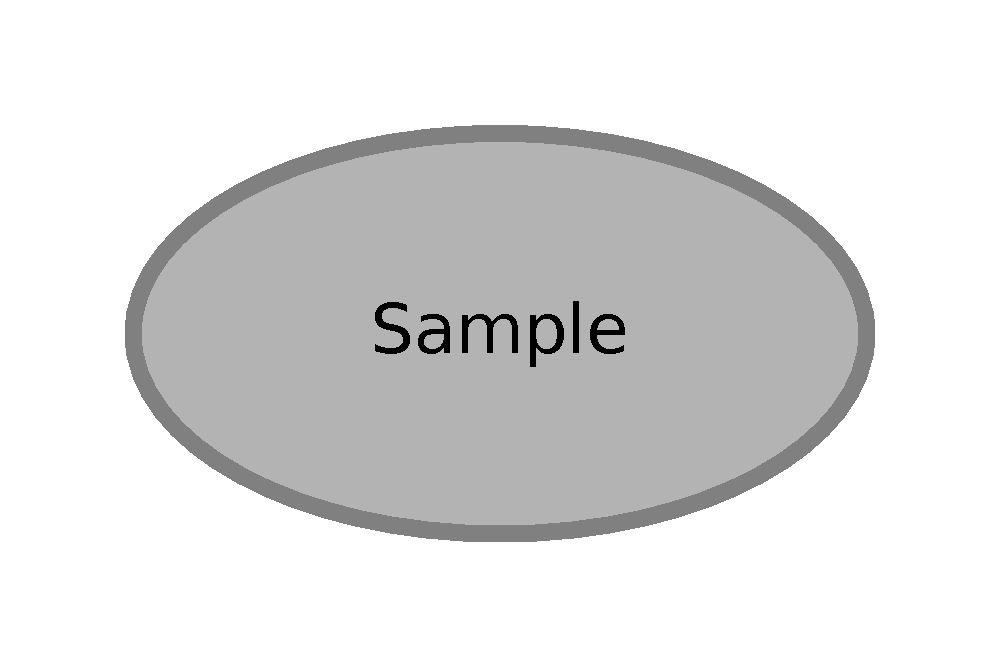
\includegraphics[width=40mm]{sample2.pdf}
  \end{center}
  \caption{sample fig2}
  \label{fig:2}
 \end{minipage}
\end{figure}

\newpage

\section{items}
sumple items.
\begin{itemize}
 \item[*] item 1
 \item[+] item 2
 \item[L] item 3
\end{itemize}

\section{table}
sumple table \ref{tab:one}.
\begin{table}[htb]
 \begin{center}
  \caption{test tab}
  \label{tab:one}
  \begin{tabular}[htb]{|p{4cm}|p{10cm}|} \hline
test tab & testes \\ \hline \hline
test test & testes \\ \hline
test testt & testttttttttttttttttttttttttttttttttttttttttttttttttttttttttttttt\\ \hline
test & testest\\ \hline
  \end{tabular}
 \end{center}
\end{table}

\section{dynamic font size}
\noindent \Large Large\\
\tiny tiny\\
\normalsize normal\\

\section{Reference}
Reference is this\cite{test}.

\begin{thebibliography}{99}
\bibitem{test}
test reference\\
\verb|http://www.test/index.html|
\end{thebibliography}

\end{document}